\chapter{Basic components}

In this chapter, the solutions of the first tutorial tasks, which consisted in implementing an operational amplifier schematic in Cadence and a clock generator in Verilog, are described.

\section{Operational amplifier}

The first task was to implement an operational amplifier. The schematics of the differential stage and bias circuit of the OpAmp were provided. The implemented amplifier can be found in the file (\texttt{OpAmp}). The simulation results given in figure ~\ref{fig:opAmpSimulation} are obtained in Cadence with the following testbench (Table 
~\ref{table:opAmpTestbench}): 

\begin{table}[!h]
	\centering
	\begin{tabular}{|l|l|l|}
		\hline
		Name & Type & Value \\
		\hline
		$V_{dd}$ & constant & 1.2V \\
		$V_{ref}$, $V_{bias}$, $V_{-}$ & constant & 600mV \\
		$V_{+}$ (In) & pulse & AC=500mV, DC=0V, f=1MHz \\
		\hline
	\end{tabular}
	\caption{Operational amplifier testbench}
	\label{table:opAmpTestbench}
\end{table}

As expected, the operational amplifier behaves as a comparator.

\begin{figure}[h]
	\centering
	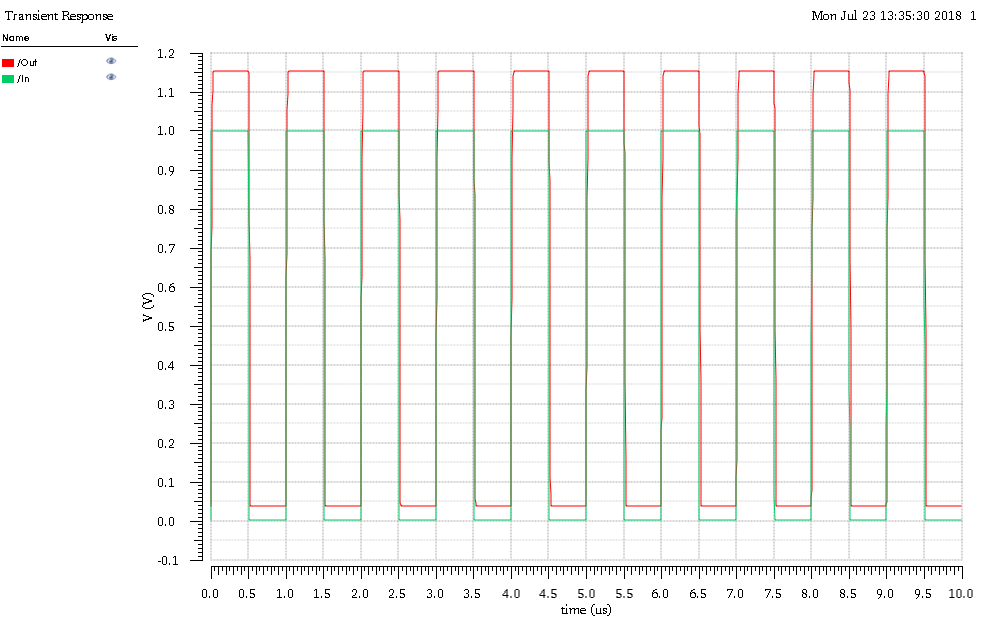
\includegraphics[scale=0.65]{images/BasicComponents/Task1OpAmpSimulation.png}
	\caption{Operational amplifier simulation}
	\label{fig:opAmpSimulation}
\end{figure} 

\section{Clock generator}

The second task consisted in implementing a clock generator (\texttt{clkGen}) in Verilog. The Verilog code was provided. The results of the simulation in ModelSim are given in figure \ref{fig:clkGenSimulation}.

\begin{figure}[h]
	\centering
	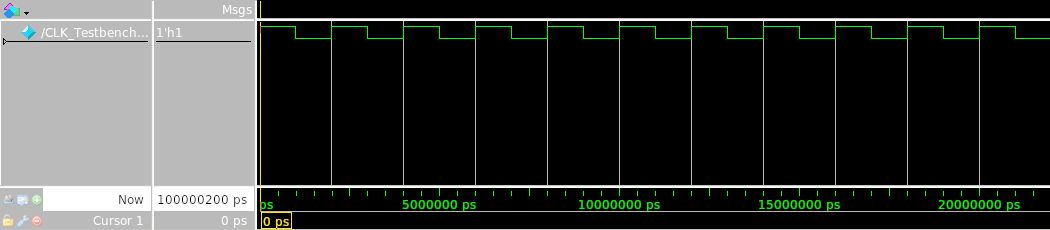
\includegraphics[scale=0.6]{images/BasicComponents/Task2ClkGenSimulation.png}
	\caption{Clock generator simulation}
	\label{fig:clkGenSimulation}	
\end{figure}

For more configurability, an additional parameter \texttt{FKHZ} was introduced, which corresponds to the desired frequency in kHz.